% Kompiuterijos katedros šablonas
% Template of Department of Computer Science II
% Versija 1.0 2015 m. kovas [ March, 2015]

\documentclass[a4paper,12pt,fleqn]{article}
\usepackage[unicode,colorlinks=false]{hyperref}


\usepackage[utf8x]{inputenc}
%

\usepackage[L7x]{fontenc}
\usepackage{times}
\usepackage{ucs}
\usepackage{tabto}

 %package to switch the language
\usepackage{etoolbox}

  %set up of the page margins
\usepackage[top=2cm, bottom=2cm, left=3cm, right=1.5cm]{geometry}

 %1.1 line spacing
\linespread{1.1}


  %page numbering at the right side
\usepackage{fancyhdr}
\pagestyle{fancyplain}
\fancyhf{}
\renewcommand{\headrulewidth}{0pt} 
\fancyhfoffset[RO]{0cm}

  %to number at the bottom (exchange lines to number at the top)
\rfoot{\thepage}
  %\rhead{\thepage} %

% \usepackage[usenames,dvipsnames]{pstricks}
\urlstyle{same}
\hypersetup{
%  citecolor=Blue,
%  linkcolor=Blue,
%  urlcolor=Blue
pdfborder={0 0 0 }
}

 %for includegraphics
\usepackage{graphicx}



\usepackage[toc,page]{appendix}


\usepackage{caption}

 %for source codes
\usepackage{listings}
\lstset{commentstyle=\color{red},xleftmargin=10pt, framexleftmargin=6pt, numbersep=1mm, frame=single, numbers=left,numberstyle=\footnotesize,extendedchars=\true, inputencoding=utf8x,basicstyle=\footnotesize,extendedchars=true,
 keywordstyle=\color{black}\bfseries, breaklines=true, breakautoindent=true,framesep=8pt,linewidth=0.95\textwidth
}

 %for algorithms
\usepackage{algorithm}
\usepackage{algorithmic}
 %instead of the above two packages we can use algorithms2e
 %\usepackage[boxed,linesnumbered,vlined,slide]{algorithm2e}

 %special symbols
\usepackage{amsfonts}
\usepackage{amssymb}
\usepackage{amsmath}

 %for theorem like environments
\usepackage{amsthm}

 \usepackage{datetime}
 \renewcommand{\dateseparator}{--}


% SI system units
\usepackage{siunitx}
\sisetup{detect-all}
% Problem with fonts \SI{x.xx}{\micro\metre}, solved with updmap-sys --enable Map=utm.map
\renewcommand{\sfdefault}{uhv}
\renewcommand{\rmdefault}{utm}
\renewcommand{\ttdefault}{ucr}

% List management (itemize, etc.)
\usepackage{enumitem}

\newcommand*{\urlw}[1]{\href{#1}%
            {\nolinkurl{#1}}}

\numberwithin{equation}{section}


\newtoggle{inLithuanian}
 %If the report is in Lithuanian, it is set to true; otherwise, change to false
\settoggle{inLithuanian}{false}
\newtheorem{exmp}{Example}[subsection]
\usepackage{tabularx}
\usepackage{listings}
\usepackage{tabu}
\usepackage{hyperref}
%create file preface.tex for the preface text
%if preface is needed set to true
\newtoggle{needPreface}
\settoggle{needPreface}{false}

\newtoggle{signaturesOnTitlePage}
\settoggle{signaturesOnTitlePage}{true}


\theoremstyle{definition}
\newtheorem{definition}{\keyWordDefinition}
\newtheorem{example}{\keyWordExample}
\def\QED{\unskip\nobreak\hfill\kern5pt$\Box$}

\iftoggle{inLithuanian}{
%\usepackage[L7x]{fontenc}
\usepackage[english,lithuanian]{babel}
\usepackage{tabu}
\newcommand{\todayiso}{\the\year \dateseparator \twodigit\month \dateseparator \twodigit\day}


\renewcommand{\today}{\number\year\space m. \space \ifcase\month\or
  sausio\or vasario\or kovo\or balandžio\or gegužės\or birželio\or
  liepos\or rugpjūčio\or rugsėjo\or spalio\or lapkričio\or
  gruodžio\fi
  \space\number\day\space d.}


 \usepackage{tocloft}
 \renewcommand\cftsecaftersnum{.} 
 \renewcommand\cftsubsecaftersnum{.} 
 \renewcommand\cftsubsubsecaftersnum{.}

 \usepackage{VUMIFKK}

 \DeclareCaptionLabelFormat{captionlt}{#2 #1}
   %smth is not fine with algorithms 
 \DeclareCaptionLabelFormat{captionltalg}{#2 #1 algoritmas}

 \usepackage{indentfirst}
 \renewcommand{\appendixtocname}{Priedai}
 \renewcommand{\appendixpagename}{Priedai}
 \renewcommand{\contentsname}{Turinys} 

 \renewcommand{\lstlistingname}{išeities kodas}
 \renewcommand{\figurename}{pav}
 \renewcommand{\tablename}{lentelė}


 \captionsetup*[lstlisting]{   
 labelsep=period,labelformat=captionlt
 }
 \captionsetup*[figure]{   
% labelsep=period,
 labelsep=space, %babel redefines pav to pav.
 labelformat=captionlt
 }
 \captionsetup*[table]{   
  labelsep=period,
  labelformat=captionlt
 }
 \renewcommand{\algorithmicrequire}{\textbf{Įvestis:}}
 \renewcommand{\algorithmicensure}{\textbf{Išvestis:}}

 \captionsetup*[algorithm]{   
 labelsep=period,labelformat=captionltalg
 }

\renewcommand{\thmhead}[3]{#2 #1#3}

}
{
%\usepackage[OT1,T1]{fontenc}
%\usepackage[L7x]{fontenc}



\usepackage[english]{babel}
\newcommand{\todayiso}{\twodigit\month \dateseparator \twodigit\day \dateseparator \the\year}
 \captionsetup*[algorithm]{   
 labelsep=period
 }
\captionsetup*[lstlisting]{   
 labelsep=period
 }
 \captionsetup*[figure]{   
 labelsep=period
 }
 \captionsetup*[table]{   
 labelsep=period
 }


}

%some kywords
 \def\keywordAbstract{\iftoggle{inLithuanian}{Santrauka}{Abstract}}
 \def\keywordAbstractOther{\iftoggle{inLithuanian}{Summary}{Santrauka}}
 \def\keyWordIntroduction{\iftoggle{inLithuanian}{Įvadas}{Introduction}}
 \def\keyWordConclusions{\iftoggle{inLithuanian}{Išvados ir rekomendacijos}{Conclusions and Recommendations}}

 \def\keyWordPreface{\iftoggle{inLithuanian}{Pratarmė}{Preface}}
 \def\keyWordAppendice{\iftoggle{inLithuanian}{Priedas}{Appendix}}
 \def\keyWordSignature{\iftoggle{inLithuanian}{parašas}{signature}}
 \def\keyWordDefinition{\iftoggle{inLithuanian}{apibrėžimas}{Definition}}
 \def\keyWordExample{\iftoggle{inLithuanian}{pavyzdys}{Example}}

\newcommand{\bothabstracts}[3]{
\setcounter{secnumdepth}{0}
\newpage
\hspace{2cm}
{\centering{\section{\keywordAbstract}}}

#1
\newpage
\hspace{2cm}
{\centering \section{\keywordAbstractOther}}

\begin{center}{\textbf{#2} }\end{center}

 #3
\setcounter{secnumdepth}{3}
}

 %non-numbered sections: #1 param: for labeling sec:#1, #2 -section title
\newcommand{\sectionWithoutNumber}[2]{\newpage
%\hspace{2cm}
\section*{#1}
\label{sec:#2}
\addcontentsline{toc}{section}{\nameref{sec:#2}}%{#3}
 }



\newcommand{\referenceSources}[1]{
\newpage
\cleardoublepage
\phantomsection
\iftoggle{inLithuanian}{
 \renewcommand{\refname}{Literatūros šaltiniai}

 \addcontentsline{toc}{section}{Literatūros šaltiniai}
 \markboth{\refname}{Literatūros šaltiniai}
 }
{

\addcontentsline{toc}{section}{References}
\markboth{References}{References}
}

\bibliographystyle{plain}
\bibliography{#1}
}



 \newcommand\authorsignature[1]{
\begin{flushright}
 \begin{minipage}[b]{0.45\textwidth}
  \centering
  \rule{\textwidth}{0.5pt}\\
   #1
  \end{minipage}
\end{flushright}
 }




 \newcommand\authorsignatures[5]{%
   \vspace{1cm}
   \authorsignature{#1}
   \ifstrequal{#2}{}{}{\vspace{0.3cm}
     \authorsignature{#2}
     \ifstrequal{#3}{}{}{\vspace{0.3cm}
      \authorsignature{#3}
      \ifstrequal{#4}{}{}{\vspace{0.3cm}
        \authorsignature{#4}
        \ifstrequal{#5}{}{}{\vspace{0.3cm}
         \authorsignature{#5}       
        }
      }
    }
} 
}

\newcommand{\authortitle}{
\iftoggle{signaturesOnTitlePage}{
\tiny{\keyWordSignature}
}{}
}

\newcommand{\depttitlepage}[8]
{
\thispagestyle{empty}
\begin{center}


\includegraphics[width=2cm]{jb_VU_zenklas}

%\vspace{-1cm}

\iftoggle{inLithuanian}
{ 
  VILNIAUS UNIVERSITETAS\\
  MATEMATIKOS IR INFORMATIKOS FAKULTETAS\\
  INFORMATIKOS INSTITUTAS\\
  KOMPIUTERINIO IR DUOMENŲ MODELIAVIMO KATEDRA
}
{ %Department of Computer Science
  VILNIUS UNIVERSITY \\
  FACULTY OF MATHEMATICS AND INFORMATICS \\
  DEPARTMENT OF COMPUTER SCIENCE\\
}

\vspace{5cm}

#1\\
\vspace{0.5cm}
\textbf{\Large #2}
\end{center}

\vspace{5cm}


\hspace{0.5\textwidth}
\begin{minipage}{0.4\textwidth}
 \begin{flushleft} 
\iftoggle{inLithuanian}
{
 \ifstrequal{#3}{}{}{Atliko:\\[5pt]}
}
{
\ifstrequal{#3}{}{}{Done by:\\[5pt]}
}

%\noindent
\begin{tabular}{@{}lr}%\setlength\tabcolsep{0pt}
\ifstrequal{#3}{}{}{#3&\hspace{2cm}\authortitle\\[5pt]}
\ifstrequal{#4}{}{}{#4&\authortitle\\[5pt]}
\ifstrequal{#5}{}{}{#5&\authortitle\\[5pt]}
\ifstrequal{#6}{}{}{#6&\authortitle\\[5pt]}
\ifstrequal{#7}{}{}{#7&\authortitle\\}
\end{tabular}

\end{flushleft}

\end{minipage}

\vspace{0.5cm}
\hspace{0.5\textwidth}
\begin{minipage}{0.4\textwidth}
 \begin{flushleft} 

\ifstrequal{#8}{}{}
{

\iftoggle{inLithuanian}
{
Vadovas:
}
{
Supervisor:
}

#8

}

\end{flushleft}

\end{minipage}


\vfill

\begin{center}
Vilnius\\
\the\year
\end{center}

\iftoggle{needPreface}{
 \sectionWithoutNumber{\keyWordPreface}{preface}
Pratarmės (Preface) informacija


\iftoggle{inLithuanian}
{
\vspace{\baselineskip}\hfill
\today
}
{
 \vspace{\baselineskip}\hfill \today
}

 \vspace{5cm}

\iftoggle{signaturesOnTitlePage}{}
{
\authorsignatures{#3}{#4}{#5}{#6}{#7}
}
}{}
\newpage
}


\begin{document}
 % #1 -report type, #2 - title, #3-7 students, #8 - supervisor
 \depttitlepage{Course Work}{Distributed File Systems}{Adomas Bazinys} 
 {}{}{}{}% students 2-5
 {Doc. Linas Bukauskas}

\tableofcontents

 %both abstracts
\bothabstracts{Goal of Distributed File System is to decentralize a network and make it more efficient by increasing files availability. Distributed File Systems were invented to make data exchanging more faster and comfortable.

This work will help to get familiar with possible types and architecture of Distributed File System. This work will focus on InterPlanetary File System and it will be analyzed in more detail. There will be also upload/download tests in this work in order to measure performance of IPFS system.}%tex-file of abstract in original language
{Paskirstytų Failų Sistemos} %if work is in LT this title should be in English
{Paskirstytųjų failų sistemų tikslas yra pilnai decentralizuoti tinklą ir padaryti jį veiksminegsniu padidinant failų prieinamumą. Šios sistemos buvo sukurtos padaryti duomenų keitimąsi greitesniu ir patogesniu.

Šis darbas padės susipažinti su egzistuojančiais paskirstytųjų failų sistemų tipais ir jų architektūra. Darbas orientuotas į IPFS (Eng. InterPlanetary File System) failų sistemą, kuri bus išanalizuota detaliau. Taip pat darbe bus pateiktas parsiuntimo - išsiuntimo testų rezultatai, kurių tikslas ištestuoti sistemos našumą.}%tex-file of abstract in other language


%keywords and notations if needed
\sectionWithoutNumber{List of Abbrevations}{keywords}{\begin{flushleft}
\textbf{DFS} - Distributed File System.
\newline
\newline
\textbf{IPFS} - InterPlanetary File System.
\newline
\newline
\textbf{DHT} - Distributed Hash Table.
\newline
\newline
\textbf{P2P} - Peer To Peer.
\newline
\newline
\textbf{DHT} - Distributed Hash Table.
\newline
\newline
\textbf{DSHT} - Distributed Sloppy Hash Table.
\newline
\newline
\textbf{FTP} - File Transfer Protocol.
\end{flushleft}}


 %Introduction section: label is sec:intro
\sectionWithoutNumber{\keyWordIntroduction}{intro}
\tab{In} the 1980s people who wanted to share data between physical machines did it slowly and uncomfortably. A method that has been used for that is known as „Sneakernet“. This is a slang term based on transferring of data and files between physical machines through devices like flash drives, hard drives, optical disks, which were physically transported between machines on foot. It was very inefficient and time consuming ~\cite{fleishman2009take}. As response to this situation, FTP system were developed for that and became popular very fast. FTP made the situation much easier, it was also far from comfortable, data still had to be replicated twice: first from the computer to the server, then from the server to the target computer ~\cite{eriksen2005comparison}. J. C. R. Licklider in 1962 has generated an idea to create a network, where all computers are able to exchange data between each other. His idea was remembered. His idea is a possible functionality of Distributed File System ~\cite{licklider1968memoriam}.

Distributed File System is a file-service system that helps to manage data files across multiple nodes or more precisely computers. The main difference between File System and Distributed File System is that on File System data is stored locally, on Distributed File System instead of storing data on a single machine, data is stored on the clusters which is a band of computers connected to each other. If you try to use data from anyone from the machines of the cluster, it will be like a data is stored on the machine you use ~\cite{ponnavaikko2009edge}.

After solving problem of inconvenient data transfer, the next stage is to get best performance capabilities. People want pages, images, videos or other important files to load instantly and we want them in high quality.

Goal of the work: Analyze IPFS DFS, its operating principles, advantages, test performance of IPFS by creating a few IPFS nodes and measuring performance of downloading and uploading some data through IPFS system.

\bigskip
Tasks:
\begin{itemize}
    \item Define and analyze DFSs overall.
    \item Define main components of IPFS system.
	\item Analyze IPFS system architecturally.
	\item Launch IPFS and measure performance.
\end{itemize}



 %the main part
\section{Distributed File Systems}
\tab{Distributed} File System is a system on mechanism by which we can implement a common file system on different independent systems or computers. The goal of Distributed File System is to have maximum transparency and high availability properties. Reliability of DFS is achieved by making a lot of certain file copies through multiple servers ensuring that a copy of file will be accessed from a user if needed ~\cite{levy1990distributed}.


\subsection{Fault tolerance}
\tab{An} error in a computer or a communication could cause a troubles in file transferring. This property also affects availability of the distributed file system and also could reduce a consistency level of DFS when several users try to download a certain file ~\cite{levy1990distributed}.

\subsection{Transparency}
\tab{DFS} should not only provide high level of transparency, but also to hide details related to the distributed environment. The types of transparency specific to a DFS are shortly explained below ~\cite{mantena6306transparency}.
\begin{itemize}
    \item \textbf{Access Transparency} - content could be stored locally or distributed, with same operations.
    \item \textbf{Location transparency} - to access object there is no need to know their location.
    \item \textbf{Concurrent transparency} - concurrent control without affecting users or applications.
    \item \textbf{Replication Transparency} - maintains consistency of multiple backup copies without user noticing.
    \item \textbf{Failure Transparency} - normal users do not have to know about failures in the system, only admins should be informed know about them.
    \item \textbf{Migration transparency} - movement of objects must be invisible to the users of a system.
    \item \textbf{Performance transparency} - if reconfiguration is needed then it do not have to influence an instant performance of a system.
    \item \textbf{Scaling transparency} - system and apps can expand in scale without changing system structure or application programs.
    \end{itemize}

\subsection{Replication}
\tab{Replication} of documents on various machines in a DFS helps to enhance file accessibility. It has also a huge impact on performance: choosing a nearby copy of a certain file reduces a file service time. The accessibility of one replica is not influenced by the accessibility of other replicas of the file in a network. It is desirable to hide the details of replication from users. Mapping a replicated file name to a particular replica is the task of the naming scheme ~\cite{levy1990distributed}.

\subsection{Synchronization}

\tab{Purpose} of synchronization is to make sure that when file is updated, then all replicas of that data is updated in Distributed File Systems. Replica synchronization ensures that the file is updated as many times as it is altered.~\cite{vini2015novel}. There are three methods for synchronization ~\cite{depardon2013analysis}:
\begin{itemize}
\item Synchronous method blocks all requests of data until all copies of file is not updated.
\item Asynchronous method is opposite to synchronous because it allows to modify a data even if all the copies are not update.
\item The semi-asynchronous method blocks requests until certain copies are updated, but not all. This method limits access to old data in the system.
\end{itemize}

\subsection{Naming}

\tab{Names} are all sources of DFS that consist of computers, services, users, and remote objects. A DFS must make sure that objects are named orderly and clear ~\cite{levy1990distributed}.


\section{Structure of Distributed File System}

\tab{DFSs} is designed to use less hardware resources as possible. Thousands of hardware resources are used to achieve this characteristic by combining their resources to one big file share system. DFSs provide a lot of advantages in file management. Design of DFS is created to provide file exchange services to clients. Clients are able to manipulate with files by reading, creating, deleting, writing files. System which is able to perform such an operations could be considered as distributed file system ~\cite{levy1990distributed}. This section will be based on information from Tannenbaums book.
\bigskip

There are three structures that DFS can be based on ~\cite{tanenbaum2007distributed}: 
\begin{itemize}
\item Server-Client based structures.
\item Cluster-based structures.
\item Symmetric structures.
\end{itemize}

\subsection{Server-Client based structures}
\tab{The} first figure is remote access model (see\ \ref{pav01}~Fig.) representing Server-Client based structure, where an interface with various file operations is provided by a client. File sharing operations are carried out using that interface. The server is responsible for giving an answer to those requests. In such a model file is available only on server: clients send commands to server and get work done ~\cite{levy1990distributed}. 
\bigskip
\begin{figure}[ht!]
    \centering
    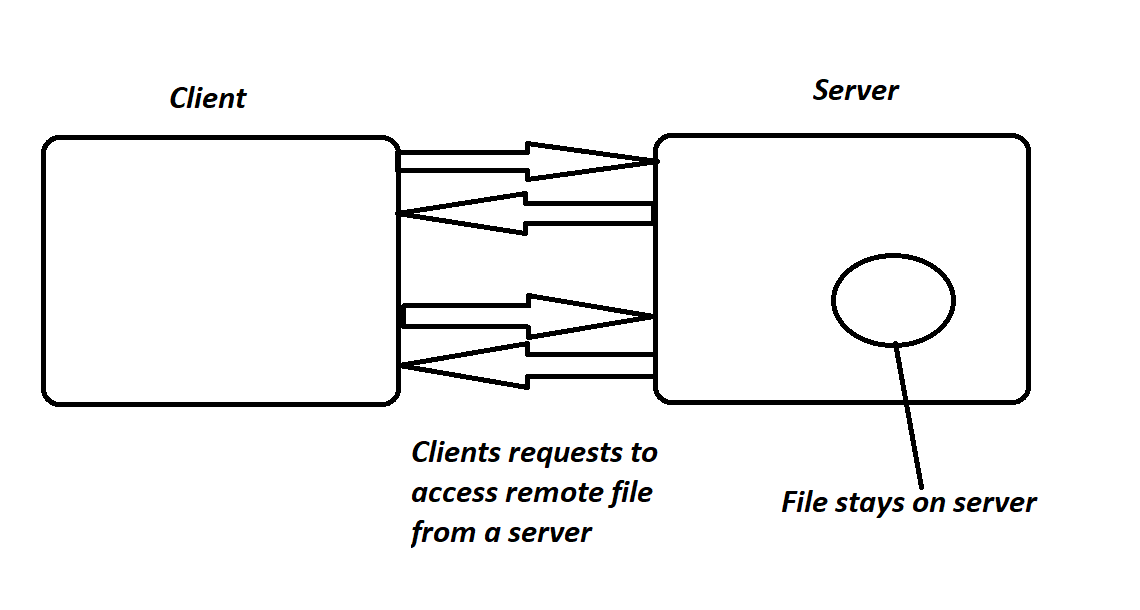
\includegraphics[clip=true, width=0.7\textwidth]{Remote_access_model.PNG}
    \caption{The remote access model.}
    \label{pav01}
\end{figure}

The second figure is Upload/Download model (see\ \ref{pav02}~Fig.) representing Server-Client based structure. Feature that separates Upload/Download and Remote-Access is that Upload/Download model download the file that client will work on, and will download file to the local file system. In this model client downloads file, works on it, and writes it back on the server following a simple and good performance ~\cite{levy1990distributed}.

\begin{figure}[ht!]
    \centering
    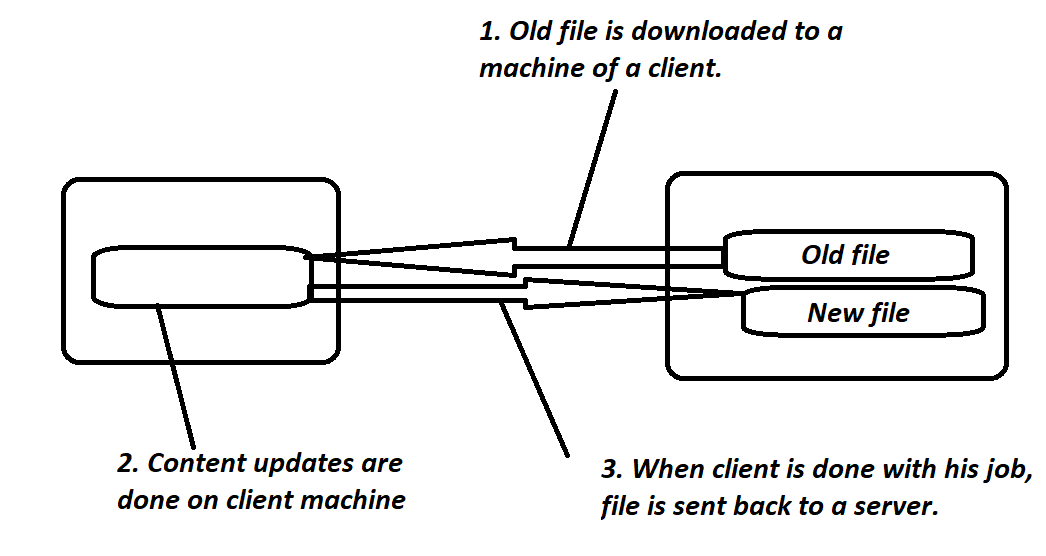
\includegraphics[clip=true, width=0.7\textwidth]{UploadDownloadModel.PNG}
    \caption{Upload/Download model.}
    \label{pav02}
\end{figure}

These both models are of server-client based structure and have a certain benefits. The Upload/Download model is not so time consuming because it requires to send only two requests to the server to work on particular file: first when you download a file and a second when you send an updated file back to the server. So, it saves server resources and provides better performance. Another useful benefit of this model is that you can use a file even if you cannot access the server. A disadvantage of downloading file to the local system and then sending it back to the server is that concurrent modification of a file by different clients can cause problems.

The Remote-Access model provides a possibility for the file server to order all operations and allow concurrent modifications to the files. A disadvantage of this model is that client could use a files if it can connect to the file server. If there will be no connection to the server then client will be not able to access the files.

\subsection{Cluster-based architecture}
\tab{DFS} with cluster-based architecture do not store data on a single server. There are multiple servers in such a system. One of them is the master server. The purpose of this server is to store the metadata of data. All other servers are chunk servers. With having more than one server, Chunk could handle multiple clients at the same time. Using such an architecture, very large data can be processed. Example of cluster-based structure could be a Google File System ~\cite{levy1990distributed} (see\ \ref{pav03}~Fig.).
\begin{figure}[ht!]
    \centering
    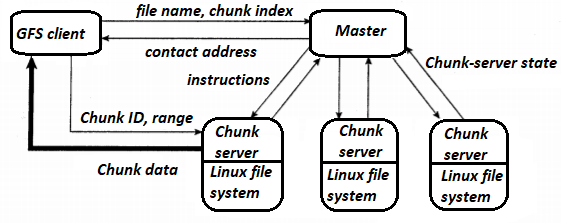
\includegraphics[clip=true, width=0.7\textwidth]{Clustered-based_architecture.PNG}
    \caption{Cluster-based architecture.}
    \label{pav03}
\end{figure}

\subsection{Symmetric architecture}

\tab{Fully} distributed file systems also known as decentralized do not have servers. It means that such a systems are made up from a lot of nodes which shares data between each other. Majority of systems use Distributed Hash Table (DHT) approach for distributing data between nodes. An example of such an architecture could be Ivy Distributed File System (see\ \ref{pav04}~Fig.). It consists of three layers: the first layer is distributed hash table used to generate hash of files, the middle layer which is fully distributed block-oriented storage layer and third layer which spans a whole file system ~\cite{levy1990distributed}.

\begin{figure}[ht!]
    \centering
    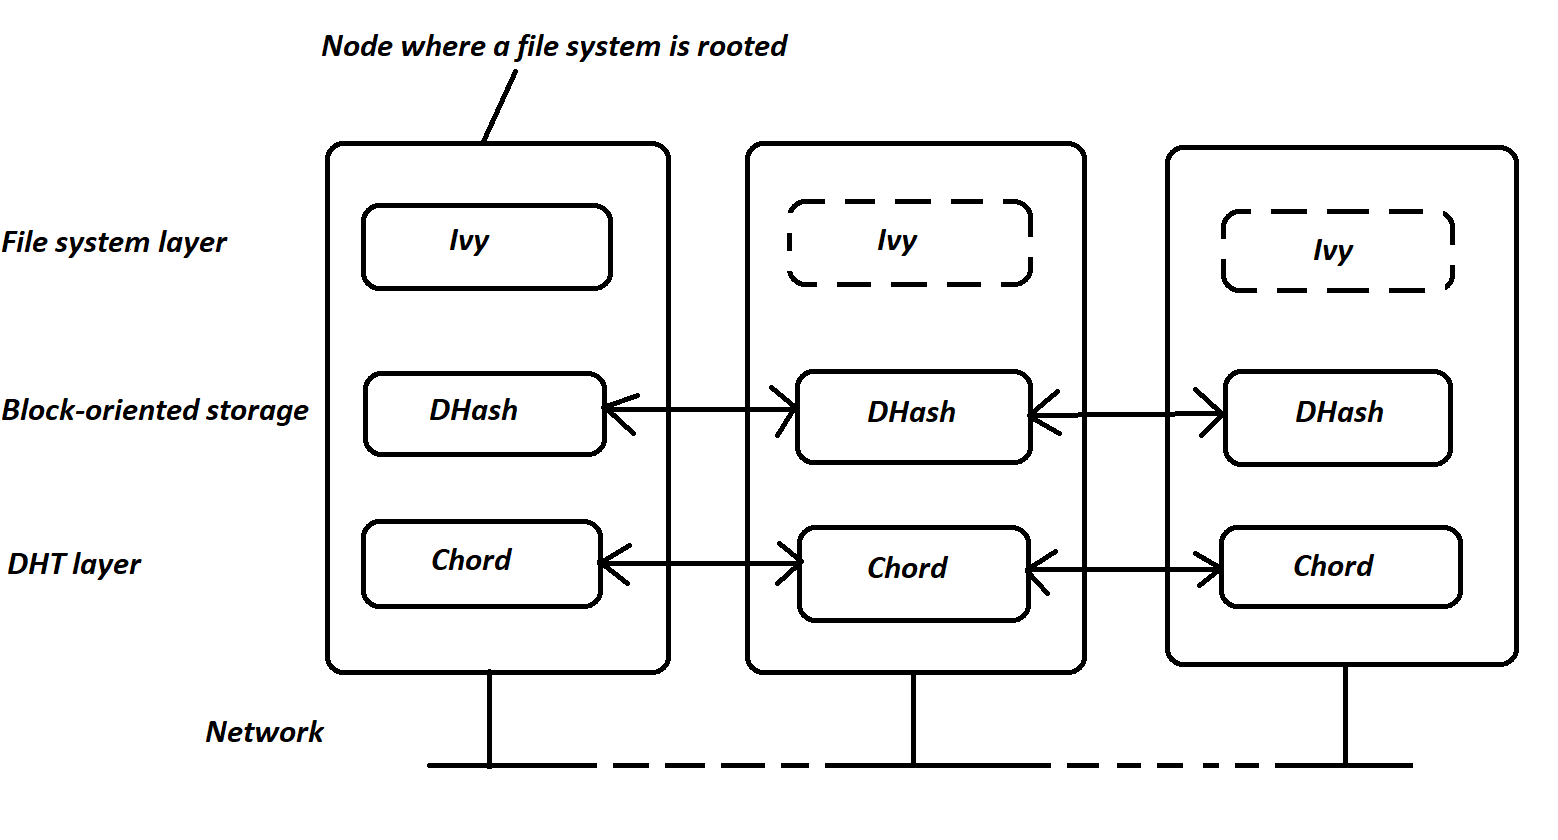
\includegraphics[clip=true, width=0.7\textwidth]{Ivy_DFS.PNG}
    \caption{Symmetric architecture.}
    \label{pav04}
\end{figure}


\section{Introduction to Interplanetary File System}

\tab{IPFS} is known as InterPlanetary File System. The development of this system was not started from a base. IPFS combines ideas from previous p2p systems like BitTorrent, Git and Kademlia DHT. Developers wanted this system to become a change of systems such as HTTP. IPFS and HTTP are compared below(see \ref{pav05}~Fig.) ~\cite{PVipfs}. All members of IPFS are known as nodes. IPFS file sharing takes place directly between nodes. IPFS is a p2p system without servers. The main difference between these two systems is that IPFS do not have server, and HTTP has it ~\cite{benet2014ipfs}.

\begin{figure}[ht!]
    \centering
    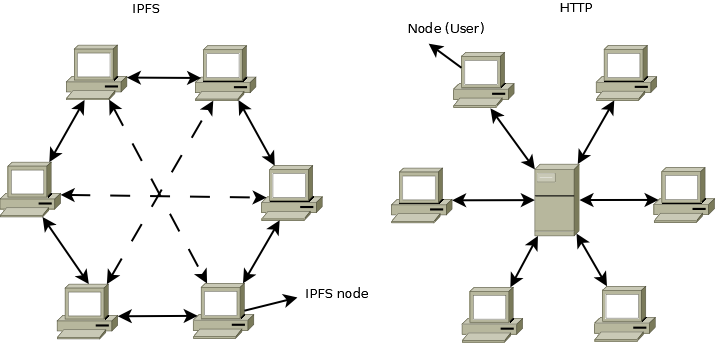
\includegraphics[clip=true, width=0.7\textwidth]{ipfsVShttp.PNG}
    \caption{Difference between IPFS and HTTP.}
    \label{pav05}
\end{figure}

\subsection{Developers of IPFS}
\tab{Juan} Benet and company Protocols Labs are founders of IPFS system. The development of system was started in 2014 and being developed up to now \cite{JuanBenetInfo}.

\section{Definitions}
\tab{This} section will help you to get familiar with the definitions used in this work.


\subsection{Data Addressing}
\tab{HTTP} is a mechanism used for data addressing with URLs. In IPFS system data addressing is carried out using contents hash. 

\subsubsection{HTTP data addressing}
\tab{Hostname}, port, path and the filename are used to address data in HTTP ~\cite{HTTP}. For example, if the location of a certain file is changed, and no other page was created for that link, then that link becomes unreachable.

\subsubsection{IPFS data addressing}
\tab{Files} in IPFS can be accessed by using the content hash. Content hash is used to build the link to files. If we add a file to IPFS, the certain hash will be assigned to that file. IPFS provides an ability to change files content (Git property) ~\cite{benet2014ipfs}. For example, if we add a file X.txt with a content of "I like IPFS" and getting a hash of it, then change a content to "I like IPFS very much" and adding it one more time to IPFS then a new hash will be created. The both versions of file including old and new will be still available only with separate hashes. That will be demonstrated in \textbf{7.2} section.

\begin{exmp} IPFS hash example
\begin{center}
	https://ipfs.io/ipfs/\textbf{QmR7GSQM93Cx5eAg6a6yRzNde1FQv7uL6X1o4k7zrJa3LX}
\end{center}
\end{exmp}

\subsection{Multiformats}
\tab{Multiformat} is a set of protocols/formats used in IPFS. They role is to try to extend existing formats by adding self-describing components. Two formats that are part of the IPFS structure are \textbf{Multihash} and \textbf{Multiaddr} ~\cite{multiformats}.

\subsubsection{Multihash}
\tab{Multihash} is a multiformat or protocol/format maintained and developed by Protocol Labs company. This multihash hash function is used for IPFS Hashes encoding. Every hash-key consists of it and two additional values: the function code of the hash function used to create this hash and the length of hash. IPFS nodes use sha2-256 hash function. After generating multihash it will be encoded by Base58 ~\cite{multihash}.
\begin{exmp} IPFS hash example
\begin{center}
\begin{tabu} to 0.8\textwidth { | X[c] | X[c] | X[c] | }
 \hline
 \textbf{sha2-256} & \textbf{size} & \textbf{sha2-256("hello ipfs")} \\
 \hline
 0x12  & 0x20  & String multiHash  \\
\hline
\end{tabu}
\newline
\newline
\begin{flushleft}
multiHash = "\textbf{4779eac1a794c2777e06cd6300e8faa3801b0591a291e581f2d6a20c19fd38da}"
\newline
After concatenating that three columns it will be: 
\newline
concated = "\textbf{12204779eac1a794c2777e06cd6300e8faa3801b0591a291e581f2d6a20c19fd38da}"
\newline
After encoding it to Base58 it will be:
\newline
finalHash = "\textbf{QmT9fUoLK3juU5drvgSomPxNDiJZuzmH4sYpYhVyDNFefB}"
\end{flushleft}

\end{center}
\end{exmp}

\subsubsection{Multiaddr}

\tab{Multiaddr} is way to express network addresses to a different combinations and is mostly used in nodes addressing. Similarly as in multihash every function has its own function code, in Multiaddr every protocol represents a function code ~\cite{multiaddr}.

\begin{exmp}
Typical form: \newline \textbf{/ip4/127.0.0.1/udp/1234}\newline
Multiaddr form: \newline \textbf{0x4 0x7f 0x0 0x0 0x1 0x91 0x2 0x4 0xd2}.
\end{exmp}

\section{Mostly used IPFS commands in Linux terminal}

\tab{As} we already know IPFS allows us to share and get (download) desirable content. Linux terminal provides an ability to execute IPFS commands quickly and comfortably. Before executing any IPFS statement it is necessary to initialize IPFS configuration and start a daemon processes which are needed to start working with IPFS.

\begin{exmp} Initialization of IPFS node and starting of daemon process.
\newline
\$ ipfs init \&&\&& ipfs daemon
\end{exmp}


To add or get data from IPFS system user has to perform \textbf{add} and \textbf{get} commands respectively. Lets say we have a text file \textbf{test.txt} with a content of "hello ipfs".


\begin{exmp} Example of adding data to IPFS.
\begin{lstlisting}[caption={Adding data to IPFS.},label={abc}]
ipfs add test.txt
added QmSoASxb8aNVGk3pNWpZvXEZTQKxjGeu9bvpYHuo5bP1VJ test.txt
\end{lstlisting}
As we see hash of the file is generated.
\end{exmp}

\begin{exmp} Example of getting data from IPFS.

\begin{lstlisting}[caption={Getting data from IPFS.},label={abc}]
ipfs get QmSoASxb8aNVGk3pNWpZvXEZTQKxjGeu9bvpYHuo5bP1VJ
ls
QmSoASxb8aNVGk3pNWpZvXEZTQKxjGeu9bvpYHuo5bP1VJ
\end{lstlisting}
After get command is successfully executed the requested file will appear in a current directory as we see and also it could be accessed from a browser: 
\newline
\textbf{\url{https://ipfs.io/ipfs/QmSoASxb8aNVGk3pNWpZvXEZTQKxjGeu9bvpYHuo5bP1VJ}}
\end{exmp}

\section{IPFS-Architecture}

\subsection{Identities}
\tab{Identities} sub-protocol is responsible for the node identity and verification of IPFS nodes. When the IPFS node is initialized, then a 2048-bit RSA key pair(public and private keys) is created. Public key hash is generated using a multihash function and then this hash is assigned to a NodeID ~\cite{identity}.

\subsubsection{Communication between Nodes}
\tab{When} a first node tries to establish relationship with second node, both nodes exchange NodeID and Public key. First node generates hash of the second node public key and if that hash is not the same as NodeID of a second node than connection between these two nodes will be interrupted ~\cite{benet2014ipfs}.

\subsection{libp2p - PeerToPeer library}
\tab{This} p2p library holds a content used for \textbf{network} connectivity between nodes, \textbf{routing}(data lookup) in the network and data \textbf{exchange} between nodes ~\cite{libp2p}.

\subsubsection{Network}

\tab{This} layer is responsible for connection to other nodes in the IPFS file system. Goal of this libp2p part is to get the maximum IPFS node availability level over the whole IPFS network ~\cite{benet2014ipfs}. 

\subsubsection{Routing}

\tab{Routing} provides an opportunity to get a specific network addresses of other IPFS nodes that can provide desirable data.

The routing module of node gets a hash-key and get respond with the list of one or more node info objects which contain a NodeID and multiaddr addresses of that node. This data is used for contacting the other IPFS nodes ~\cite{benet2014ipfs}.
\newline

\textbf{Distributed Hash Table}
\newline

 Distributed Sloppy Hash Table (DSHT) is used to hold hash key value of NodeIDs pairs. It is distributed on all active IPFS nodes. It means that every node will be responsible for a certain part of all blocks added to IPFS. If IPFS node has no more connection to IPFS, then the responsibility of his part of the DHT is given to other node ~\cite{benet2014ipfs}. 

Files are stored inside IPFS objects and these objects can store up to 256 kilobytes worth of data. 

If file is bigger than 256KB like a video or image then that file is split up into multiple IPFS objects that are all 256 kilobytes size. After that the system will create an empty IPFS object that links to all the other pieces of the file. If more technically for every object new entry with content of a block hash with reference to a NodeID is added to DHT. 

\begin{exmp} Example of adding a file bigger than one IPFS object size (256kb).

\begin{lstlisting}[caption={Requesting IPFS objects of file > 256kb.},label={abc}]
ipfs get object QmdJTmCxwcpoGbEVfT6b9j4RZJWNcF2GQG1Ajf9XB6XtVP
\end{lstlisting}
\textbf{And in a output we get:}
\begin{lstlisting}[caption={Created IPFS objects of file > 256kb.},label={abc}]
"Links":[
{"Name":"","Hash":"QmTi2QvnQgwdnQEide1GtZ4WrmJgrxerzTp4MNei9UJC2w","Size":262158},
{"Name":"","Hash":"QmZpwJYecK6xYw8P9YsJyRo5a7LJFEckHEXxSqP178vQyJ","Size":262158},
{"Name":"","Hash":"QmdQUyndMnU9sXAvPbNNZbphWBfGWoLB7wHg4NGm7VpWkf","Size":255406}],
"Data":"\u0008\u0002\u0018\ufffd\ufffd/ \ufffd\ufffd\u0010 \ufffd\ufffd\u0010 \ufffd\ufffd\u000f"}
\end{lstlisting}

\end{exmp}

For example, text file with the content of "hello ipfs" can be stored in a single IPFS object because its size do not exceed 256KB. A new entry with content of block hash with reference to File is added to DHT.

\begin{exmp} Example of adding a file which size is less than one IPFS object size (256kb). We will use the same test.txt file used for examples in previous section.
\begin{lstlisting}[caption={Requesting IPFS objects of file < 256kb.},label={abc}]
ipfs get object QmSoASxb8aNVGk3pNWpZvXEZTQKxjGeu9bvpYHuo5bP1VJ
\end{lstlisting}
\textbf{And in a output we get:}
\begin{lstlisting}[caption={Created IPFS objects of file < 256kb.},label={abc}]
{"Links":[],
"Data":"\u0008\u0002\u0012\u000bhello ipfs\n\u0018\u000b"}
\end{lstlisting}
\end{exmp}

\subsubsection{Exchange}
IPFS distributed file system can use a lot of exchange protocols. The mostly used protcol in IPFS is BitSwap. BitSwap is used to perform data transfer between the IPFS nodes. BitSwap functionality consists of such a steps:
\begin{enumerate}
    \item 	Requester IPFS node asks for a certain part of file to download.
    \item 	That file is added to want list of that first IPFS node.
    \item 	BitSwap module sends that want list to other nodes that have some parts of that file according to DHT.
    \item 	That nodes put their having parts of data to the have list.
    \item 	If one of that nodes has that file that the first node wanted to download then that part of data is sent to requester node.
    \item 	At the moment when desired part of data is sent all other nodes will stop searching for data.
    \item 	Want list and have list are eliminated.
\end{enumerate}

\section{Related work}

\tab{As} mentioned in the beginning, the purpose of this work is to focus on IPFS performance. We will do a simple download test case which is written in Bash language. We have five Ubuntu 16.04 virtual machines with IPFS installed. Goal is to test IPFS performance by choosing a different number of requests and delays between them. For defining performance test results, we will use average request execution time variables. We will perform three tests:

\begin{itemize}
    \item 5 requests to the file with delay which is equal to 0 seconds. It means that we will send 5 requests to the file without interrupts.
    \item 5 requests to the file with delay which is equal to 5 seconds. It means that we will send 5 requests to the file every five second.
    \item 5 requests to the file with delay which is equal to 10 seconds. It means that we will send 5 requests to the file every ten seconds.
\end{itemize}

After this test we will check difference between all three download speed averages.

\subsection{Download Experiment}

\begin{lstlisting}[caption={Download test with delay which is equal to 0 seconds.},label={abc}]
Saving file(s) to QmR7GSQM93Cx5eAg6a6yRzNde1FQv7uL6X1o4k7zrJa3LX
208.44 KB / 208.44 KB  100.00% 0s

Download time of IPFS_NODE1: 1.313395512 seconds
Saving file(s) to QmR7GSQM93Cx5eAg6a6yRzNde1FQv7uL6X1o4k7zrJa3LX
0 B / 208.44 KB    0.00%
208.44 KB / 208.44 KB  100.00% 0s
Download time of IPFS_NODE2: 1.449446200 seconds
Saving file(s) to QmR7GSQM93Cx5eAg6a6yRzNde1FQv7uL6X1o4k7zrJa3LX
208.44 KB / 208.44 KB  100.00% 0s

Download time of IPFS_NODE3: 1.277026253 seconds
Saving file(s) to QmR7GSQM93Cx5eAg6a6yRzNde1FQv7uL6X1o4k7zrJa3LX
208.44 KB / 208.44 KB  100.00% 0s

Download time of IPFS_NODE4: 3.003086492 seconds
Saving file(s) to QmR7GSQM93Cx5eAg6a6yRzNde1FQv7uL6X1o4k7zrJa3LX
0 B / 208.44 KB    0.00%
208.44 KB / 208.44 KB  100.00% 0s
Download time of IPFS_NODE5: 1.050746487 seconds

Average download speed of all download processes in kb/s:
146.70291
\end{lstlisting}    

Result of this test is that average download speed of all five requests is \textbf{146.70291} kb/s.

\newpage
\begin{lstlisting}[caption={Download test with delay which is equal to 5 seconds.},label={abc}]
Saving file(s) to QmR7GSQM93Cx5eAg6a6yRzNde1FQv7uL6X1o4k7zrJa3LX
0 B / 208.44 KB    0.00%
208.44 KB / 208.44 KB  100.00% 0s
Download time of IPFS_NODE1: .931403434 seconds
Saving file(s) to QmR7GSQM93Cx5eAg6a6yRzNde1FQv7uL6X1o4k7zrJa3LX

208.44 KB / 208.44 KB  100.00% 0s
Download time of IPFS_NODE2: .834524438 seconds
Saving file(s) to QmR7GSQM93Cx5eAg6a6yRzNde1FQv7uL6X1o4k7zrJa3LX
0 B / 208.44 KB    0.00%
208.44 KB / 208.44 KB  100.00% 0s
Download time of IPFS_NODE3: 1.158473146 seconds
Saving file(s) to QmR7GSQM93Cx5eAg6a6yRzNde1FQv7uL6X1o4k7zrJa3LX
0 B / 208.44 KB    0.00%
208.44 KB / 208.44 KB  100.00% 0s
Download time of IPFS_NODE4: 5.835610128 seconds
Saving file(s) to QmR7GSQM93Cx5eAg6a6yRzNde1FQv7uL6X1o4k7zrJa3LX
208.44 KB / 208.44 KB  100.00% 0s

Download time of IPFS_NODE5: 2.079382666 seconds

Average download speed of all download processes in kb/s:
157.88973
\end{lstlisting}    

In this test we can see that average download speed is equal to \textbf{157.88973} kb/s.

\begin{lstlisting}[caption={Downlaod test with delay which is equal to 10 seconds.},label={abc}]
Saving file(s) to QmR7GSQM93Cx5eAg6a6yRzNde1FQv7uL6X1o4k7zrJa3LX
208.44 KB / 208.44 KB  100.00% 0s

Download time of IPFS_NODE1: 1.318359470 seconds
Saving file(s) to QmR7GSQM93Cx5eAg6a6yRzNde1FQv7uL6X1o4k7zrJa3LX
0 B / 208.44 KB    0.00%
208.44 KB / 208.44 KB  100.00% 0s
Download time of IPFS_NODE2: .902398822 seconds
Saving file(s) to QmR7GSQM93Cx5eAg6a6yRzNde1FQv7uL6X1o4k7zrJa3LX

208.44 KB / 208.44 KB  100.00% 0s
Download time of IPFS_NODE3: 1.534072257 seconds
Saving file(s) to QmR7GSQM93Cx5eAg6a6yRzNde1FQv7uL6X1o4k7zrJa3LX
208.44 KB / 208.44 KB  100.00% 0s

Download time of IPFS_NODE4: 1.293983729 seconds
Saving file(s) to QmR7GSQM93Cx5eAg6a6yRzNde1FQv7uL6X1o4k7zrJa3LX

208.44 KB / 208.44 KB  100.00% 0s
Download time of IPFS_NODE5: 1.671444723 seconds

Average download speed of all download processes in kb/s:
162.15079
\end{lstlisting}    

As seen in the example the average download speed is \textbf{162.15079} kb/s.

\subsection{Results of Download Experiment}
\tab{As} we can see by increasing the delay between downloads, the average download speed is increasing. This means that it is harder for the system to distribute the files continuously requesting to download a file. Increasing delay file download speed becomes faster. It is also necessary to take into account the speed of the internet, because results can be completely different when internet speed changes.




\subsection{Upload Experiment}
\tab{To} test performance of a system, it is logical to test not only speed of download process but also how fast system is able to upload data. Now we will measure it by average upload time. We will perform such a test case:

\begin{itemize}
    \item 5 requests to upload a file with delay which is equal to 0 seconds. Five requests will be sent  without interrupts.
    \item 5 requests to upload a file with delay which is equal to 5 seconds. Five requests will be sent every 5 seconds.
    \item 5 requests to upload a file with delay which is equal to 10 seconds. Five requests will be sent every 10 seconds.
\end{itemize}

\begin{lstlisting}[caption={Upload test without delay.},label={abc}]
Please enter a delay of each upload process
0
Please enter a number of upload processes
5

added QmXr4EEva2mz3U1uJ5DfhonRdNcghkCsLyr9sdSgmwVUpj test.txt
added QmSmvKc3hu3riNzneobQuQ3ZkaAw7oRKuJz5KxyQEqQkn2 

added QmSw4k8zvbxrFWWT5B9MHLuQ2xPunbdJBxAtWWsXt5e5og test.txt
added QmNWmLXn2cGoPetjVP8y4nrf9S4HnQm15Li8igaGRXFoP1 

added QmbScFm2rSvbReKUornBJVMgakaqJYm4ZD2mTTamyXNZrj test.txt
added QmVCBfdAdybJcPTuQFqWGwqCBLXwtVLeXWPTwZPM2HK7Rb 

added QmV2UFkxh4S5YMQysXExAtZqCyYwyvnzo1rP8FdpKyuQKt test.txt
added QmXCaQnkeCDy4mf9DVtzU1NH5f2rMfNquYGR3YaAbymrUn 

added QmPQttZb6F3a1i8rLv3EJ8AK36uMQtRximpR9mqbN5WUMt test.txt
added QmPVvZGc4RAeroHVKYvjPrBW821w1BMcXz7FuwLCqyQHj9 

Sum of all upload processes: 6.558775291

Average upload speed of all processes: 1.31175
\end{lstlisting}    

As we see the average of all upload processes is \textbf{1.31175} seconds.

\newpage
\begin{lstlisting}[caption={Upload test with delay which is equal to 5 seconds.},label={abc}]
Please enter a delay of each upload process
5
Please enter a number of upload processes
5

added QmXr4EEva2mz3U1uJ5DfhonRdNcghkCsLyr9sdSgmwVUpj test.txt
added QmSmvKc3hu3riNzneobQuQ3ZkaAw7oRKuJz5KxyQEqQkn2 

added QmSw4k8zvbxrFWWT5B9MHLuQ2xPunbdJBxAtWWsXt5e5og test.txt
added QmNWmLXn2cGoPetjVP8y4nrf9S4HnQm15Li8igaGRXFoP1 

added QmbScFm2rSvbReKUornBJVMgakaqJYm4ZD2mTTamyXNZrj test.txt
added QmVCBfdAdybJcPTuQFqWGwqCBLXwtVLeXWPTwZPM2HK7Rb 

added QmV2UFkxh4S5YMQysXExAtZqCyYwyvnzo1rP8FdpKyuQKt test.txt
added QmXCaQnkeCDy4mf9DVtzU1NH5f2rMfNquYGR3YaAbymrUn 

added QmPQttZb6F3a1i8rLv3EJ8AK36uMQtRximpR9mqbN5WUMt test.txt
added QmPVvZGc4RAeroHVKYvjPrBW821w1BMcXz7FuwLCqyQHj9 

Sum of all upload processes: 5.534382174

Average upload speed of all processes: 1.10687
\end{lstlisting}    

In this case average of upload processes is \textbf{1.10687} seconds.

\begin{lstlisting}[caption={Upload test with delay which is equal to 10 seconds.},label={abc}]
Please enter a delay of each upload process
10
Please enter a number of upload processes
5

added QmXr4EEva2mz3U1uJ5DfhonRdNcghkCsLyr9sdSgmwVUpj test.txt
added QmSmvKc3hu3riNzneobQuQ3ZkaAw7oRKuJz5KxyQEqQkn2 

added QmSw4k8zvbxrFWWT5B9MHLuQ2xPunbdJBxAtWWsXt5e5og test.txt
added QmNWmLXn2cGoPetjVP8y4nrf9S4HnQm15Li8igaGRXFoP1 

added QmbScFm2rSvbReKUornBJVMgakaqJYm4ZD2mTTamyXNZrj test.txt
added QmVCBfdAdybJcPTuQFqWGwqCBLXwtVLeXWPTwZPM2HK7Rb 

added QmV2UFkxh4S5YMQysXExAtZqCyYwyvnzo1rP8FdpKyuQKt test.txt
added QmXCaQnkeCDy4mf9DVtzU1NH5f2rMfNquYGR3YaAbymrUn 

added QmPQttZb6F3a1i8rLv3EJ8AK36uMQtRximpR9mqbN5WUMt test.txt
added QmPVvZGc4RAeroHVKYvjPrBW821w1BMcXz7FuwLCqyQHj9 

Sum of all upload processes: 4.934000186

Average upload speed of all processes: 0.98680
\end{lstlisting}    

Average of upload processes in this test case is \textbf{0.98680} seconds. 

\subsection{Results of Upload Experiment}
\tab{First} thing that should be noticed in this experiment is that hash changes by every upload. We use an algorithm which changes a content of test.txt file to be able to mark it as an updated content and generate a new hash in IPFS system. As we see the average of upload times get shorter by reducing delay time. It means that it is more difficult for the system to upload a content without interrupt (with delay which is equal to 0 seconds). As in download test here is also necessary to take into account the speed of the internet, because results can be completely different when it changes.

\sectionWithoutNumber{\keyWordConclusions}{conclu}
\tab{InterPlanetary} File System is a near future technology which makes internet fully distributed and decentralized. InterPlanetary File System can be considered as a system having a consistent architecture which makes a content as available as possible. Experiments have shown that IPFS performance depends on load - the more queries to the file, the slower the content gets to the physical machine.


\referenceSources{literatureSources.bib}




\end{document}
\end{lstlisting}    
